\documentclass[twoside]{book}

% Packages required by doxygen
\usepackage{fixltx2e}
\usepackage{calc}
\usepackage{doxygen}
\usepackage[export]{adjustbox} % also loads graphicx
\usepackage{graphicx}
\usepackage[utf8]{inputenc}
\usepackage{makeidx}
\usepackage{multicol}
\usepackage{multirow}
\PassOptionsToPackage{warn}{textcomp}
\usepackage{textcomp}
\usepackage[nointegrals]{wasysym}
\usepackage[table]{xcolor}

% Font selection
\usepackage[T1]{fontenc}
\usepackage[scaled=.90]{helvet}
\usepackage{courier}
\usepackage{amssymb}
\usepackage{sectsty}
\renewcommand{\familydefault}{\sfdefault}
\allsectionsfont{%
  \fontseries{bc}\selectfont%
  \color{darkgray}%
}
\renewcommand{\DoxyLabelFont}{%
  \fontseries{bc}\selectfont%
  \color{darkgray}%
}
\newcommand{\+}{\discretionary{\mbox{\scriptsize$\hookleftarrow$}}{}{}}

% Page & text layout
\usepackage{geometry}
\geometry{%
  a4paper,%
  top=2.5cm,%
  bottom=2.5cm,%
  left=2.5cm,%
  right=2.5cm%
}
\tolerance=750
\hfuzz=15pt
\hbadness=750
\setlength{\emergencystretch}{15pt}
\setlength{\parindent}{0cm}
\setlength{\parskip}{0.2cm}
\makeatletter
\renewcommand{\paragraph}{%
  \@startsection{paragraph}{4}{0ex}{-1.0ex}{1.0ex}{%
    \normalfont\normalsize\bfseries\SS@parafont%
  }%
}
\renewcommand{\subparagraph}{%
  \@startsection{subparagraph}{5}{0ex}{-1.0ex}{1.0ex}{%
    \normalfont\normalsize\bfseries\SS@subparafont%
  }%
}
\makeatother

% Headers & footers
\usepackage{fancyhdr}
\pagestyle{fancyplain}
\fancyhead[LE]{\fancyplain{}{\bfseries\thepage}}
\fancyhead[CE]{\fancyplain{}{}}
\fancyhead[RE]{\fancyplain{}{\bfseries\leftmark}}
\fancyhead[LO]{\fancyplain{}{\bfseries\rightmark}}
\fancyhead[CO]{\fancyplain{}{}}
\fancyhead[RO]{\fancyplain{}{\bfseries\thepage}}
\fancyfoot[LE]{\fancyplain{}{}}
\fancyfoot[CE]{\fancyplain{}{}}
\fancyfoot[RE]{\fancyplain{}{\bfseries\scriptsize Generated on Sun Mar 22 2015 19\+:11\+:11 for My Project by Doxygen }}
\fancyfoot[LO]{\fancyplain{}{\bfseries\scriptsize Generated on Sun Mar 22 2015 19\+:11\+:11 for My Project by Doxygen }}
\fancyfoot[CO]{\fancyplain{}{}}
\fancyfoot[RO]{\fancyplain{}{}}
\renewcommand{\footrulewidth}{0.4pt}
\renewcommand{\chaptermark}[1]{%
  \markboth{#1}{}%
}
\renewcommand{\sectionmark}[1]{%
  \markright{\thesection\ #1}%
}

% Indices & bibliography
\usepackage{natbib}
\usepackage[titles]{tocloft}
\setcounter{tocdepth}{3}
\setcounter{secnumdepth}{5}
\makeindex

% Hyperlinks (required, but should be loaded last)
\usepackage{ifpdf}
\ifpdf
  \usepackage[pdftex,pagebackref=true]{hyperref}
\else
  \usepackage[ps2pdf,pagebackref=true]{hyperref}
\fi
\hypersetup{%
  colorlinks=true,%
  linkcolor=blue,%
  citecolor=blue,%
  unicode%
}

% Custom commands
\newcommand{\clearemptydoublepage}{%
  \newpage{\pagestyle{empty}\cleardoublepage}%
}


%===== C O N T E N T S =====

\begin{document}

% Titlepage & ToC
\hypersetup{pageanchor=false,
             bookmarks=true,
             bookmarksnumbered=true,
             pdfencoding=unicode
            }
\pagenumbering{roman}
\begin{titlepage}
\vspace*{7cm}
\begin{center}%
{\Large My Project }\\
\vspace*{1cm}
{\large Generated by Doxygen 1.8.9.1}\\
\vspace*{0.5cm}
{\small Sun Mar 22 2015 19:11:11}\\
\end{center}
\end{titlepage}
\clearemptydoublepage
\tableofcontents
\clearemptydoublepage
\pagenumbering{arabic}
\hypersetup{pageanchor=true}

%--- Begin generated contents ---
\chapter{Data Structure Index}
\section{Data Structures}
Here are the data structures with brief descriptions\+:\begin{DoxyCompactList}
\item\contentsline{section}{\hyperlink{structlokalizacja}{lokalizacja} }{\pageref{structlokalizacja}}{}
\item\contentsline{section}{\hyperlink{structslownik}{slownik} }{\pageref{structslownik}}{}
\item\contentsline{section}{\hyperlink{structslowo}{slowo} }{\pageref{structslowo}}{}
\item\contentsline{section}{\hyperlink{structwej}{wej} }{\pageref{structwej}}{}
\end{DoxyCompactList}

\chapter{File Index}
\section{File List}
Here is a list of all files with brief descriptions\+:\begin{DoxyCompactList}
\item\contentsline{section}{\hyperlink{generator_8h}{generator.\+h} }{\pageref{generator_8h}}{}
\item\contentsline{section}{\hyperlink{kontener_8h}{kontener.\+h} }{\pageref{kontener_8h}}{}
\item\contentsline{section}{\hyperlink{main_8c}{main.\+c} }{\pageref{main_8c}}{}
\item\contentsline{section}{\hyperlink{stat_8h}{stat.\+h} }{\pageref{stat_8h}}{}
\item\contentsline{section}{\hyperlink{wczytywanie_8h}{wczytywanie.\+h} }{\pageref{wczytywanie_8h}}{}
\item\contentsline{section}{\hyperlink{wypisywanie_8h}{wypisywanie.\+h} }{\pageref{wypisywanie_8h}}{}
\end{DoxyCompactList}

\chapter{Data Structure Documentation}
\hypertarget{structlokalizacja}{}\section{lokalizacja Struct Reference}
\label{structlokalizacja}\index{lokalizacja@{lokalizacja}}


{\ttfamily \#include $<$kontener.\+h$>$}

\subsection*{Data Fields}
\begin{DoxyCompactItemize}
\item 
int \hyperlink{structlokalizacja_ab3185685591101d81cb357c8117290fd}{nr}
\item 
int \hyperlink{structlokalizacja_a2900f7e89911bfea0e279125b066926b}{pref}
\item 
int \hyperlink{structlokalizacja_aec1dc6d104a7f16a3b58870e29fe48d1}{suf}
\end{DoxyCompactItemize}


\subsection{Field Documentation}
\hypertarget{structlokalizacja_ab3185685591101d81cb357c8117290fd}{}\index{lokalizacja@{lokalizacja}!nr@{nr}}
\index{nr@{nr}!lokalizacja@{lokalizacja}}
\subsubsection[{nr}]{\setlength{\rightskip}{0pt plus 5cm}int lokalizacja\+::nr}\label{structlokalizacja_ab3185685591101d81cb357c8117290fd}
\hypertarget{structlokalizacja_a2900f7e89911bfea0e279125b066926b}{}\index{lokalizacja@{lokalizacja}!pref@{pref}}
\index{pref@{pref}!lokalizacja@{lokalizacja}}
\subsubsection[{pref}]{\setlength{\rightskip}{0pt plus 5cm}int lokalizacja\+::pref}\label{structlokalizacja_a2900f7e89911bfea0e279125b066926b}
\hypertarget{structlokalizacja_aec1dc6d104a7f16a3b58870e29fe48d1}{}\index{lokalizacja@{lokalizacja}!suf@{suf}}
\index{suf@{suf}!lokalizacja@{lokalizacja}}
\subsubsection[{suf}]{\setlength{\rightskip}{0pt plus 5cm}int lokalizacja\+::suf}\label{structlokalizacja_aec1dc6d104a7f16a3b58870e29fe48d1}


The documentation for this struct was generated from the following file\+:\begin{DoxyCompactItemize}
\item 
\hyperlink{kontener_8h}{kontener.\+h}\end{DoxyCompactItemize}

\hypertarget{structslownik}{}\section{slownik Struct Reference}
\label{structslownik}\index{slownik@{slownik}}


{\ttfamily \#include $<$kontener.\+h$>$}



Collaboration diagram for slownik\+:\nopagebreak
\begin{figure}[H]
\begin{center}
\leavevmode
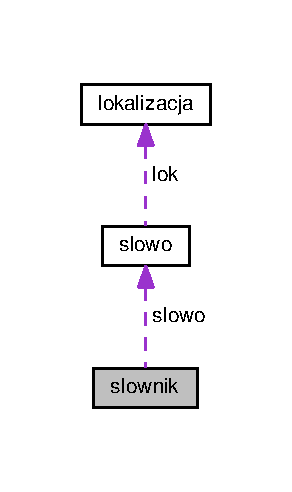
\includegraphics[width=140pt]{structslownik__coll__graph}
\end{center}
\end{figure}
\subsection*{Data Fields}
\begin{DoxyCompactItemize}
\item 
\hyperlink{kontener_8h_aac4dfae9f3beb67b30cf6fd8ddb88731}{slowo\+\_\+t} $\ast$ \hyperlink{structslownik_a512b20a3761955c3939b569f00f93716}{slowo}
\begin{DoxyCompactList}\small\item\em adres wektora przechowującego słowa \end{DoxyCompactList}\item 
int \hyperlink{structslownik_a12ee12fe22eea3f9feb644249488cabb}{miejsce}
\item 
int \hyperlink{structslownik_ad96661a61ac1dac1419dc121cfb8d565}{zajete}
\item 
int \hyperlink{structslownik_a40c60cac651b33052c12dc30918aa840}{ostatnie}
\end{DoxyCompactItemize}


\subsection{Field Documentation}
\hypertarget{structslownik_a12ee12fe22eea3f9feb644249488cabb}{}\index{slownik@{slownik}!miejsce@{miejsce}}
\index{miejsce@{miejsce}!slownik@{slownik}}
\subsubsection[{miejsce}]{\setlength{\rightskip}{0pt plus 5cm}int slownik\+::miejsce}\label{structslownik_a12ee12fe22eea3f9feb644249488cabb}
\hypertarget{structslownik_a40c60cac651b33052c12dc30918aa840}{}\index{slownik@{slownik}!ostatnie@{ostatnie}}
\index{ostatnie@{ostatnie}!slownik@{slownik}}
\subsubsection[{ostatnie}]{\setlength{\rightskip}{0pt plus 5cm}int slownik\+::ostatnie}\label{structslownik_a40c60cac651b33052c12dc30918aa840}
\hypertarget{structslownik_a512b20a3761955c3939b569f00f93716}{}\index{slownik@{slownik}!slowo@{slowo}}
\index{slowo@{slowo}!slownik@{slownik}}
\subsubsection[{slowo}]{\setlength{\rightskip}{0pt plus 5cm}{\bf slowo\+\_\+t}$\ast$ slownik\+::slowo}\label{structslownik_a512b20a3761955c3939b569f00f93716}


adres wektora przechowującego słowa 

\hypertarget{structslownik_ad96661a61ac1dac1419dc121cfb8d565}{}\index{slownik@{slownik}!zajete@{zajete}}
\index{zajete@{zajete}!slownik@{slownik}}
\subsubsection[{zajete}]{\setlength{\rightskip}{0pt plus 5cm}int slownik\+::zajete}\label{structslownik_ad96661a61ac1dac1419dc121cfb8d565}


The documentation for this struct was generated from the following file\+:\begin{DoxyCompactItemize}
\item 
\hyperlink{kontener_8h}{kontener.\+h}\end{DoxyCompactItemize}

\hypertarget{structslowo}{}\section{slowo Struct Reference}
\label{structslowo}\index{slowo@{slowo}}


{\ttfamily \#include $<$kontener.\+h$>$}



Collaboration diagram for slowo\+:\nopagebreak
\begin{figure}[H]
\begin{center}
\leavevmode
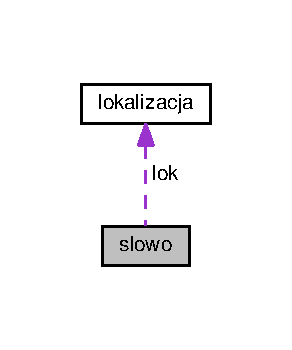
\includegraphics[width=140pt]{structslowo__coll__graph}
\end{center}
\end{figure}
\subsection*{Data Fields}
\begin{DoxyCompactItemize}
\item 
char \hyperlink{structslowo_a155485348d375daf1428b1a631808e46}{v} \mbox{[}\hyperlink{kontener_8h_aaef6c04c23aa5ab59c7530d87e355c4e}{W\+R\+D\+\_\+\+M\+A\+X\+\_\+\+L\+E\+N\+G\+H\+T}\mbox{]}
\item 
\hyperlink{kontener_8h_a973470f0d2bd5351f2f79b119fc095e8}{lok\+\_\+t} $\ast$ \hyperlink{structslowo_a8310a3996804f2f7ab2a1124b0a14617}{lok}
\item 
int \hyperlink{structslowo_ab6457a7c7e89a1b03ddd1f4282fa1a00}{miejsce}
\item 
int \hyperlink{structslowo_a7049547b2831ec4ce08c4b9419621fe8}{zajete}
\end{DoxyCompactItemize}


\subsection{Field Documentation}
\hypertarget{structslowo_a8310a3996804f2f7ab2a1124b0a14617}{}\index{slowo@{slowo}!lok@{lok}}
\index{lok@{lok}!slowo@{slowo}}
\subsubsection[{lok}]{\setlength{\rightskip}{0pt plus 5cm}{\bf lok\+\_\+t}$\ast$ slowo\+::lok}\label{structslowo_a8310a3996804f2f7ab2a1124b0a14617}
\hypertarget{structslowo_ab6457a7c7e89a1b03ddd1f4282fa1a00}{}\index{slowo@{slowo}!miejsce@{miejsce}}
\index{miejsce@{miejsce}!slowo@{slowo}}
\subsubsection[{miejsce}]{\setlength{\rightskip}{0pt plus 5cm}int slowo\+::miejsce}\label{structslowo_ab6457a7c7e89a1b03ddd1f4282fa1a00}
\hypertarget{structslowo_a155485348d375daf1428b1a631808e46}{}\index{slowo@{slowo}!v@{v}}
\index{v@{v}!slowo@{slowo}}
\subsubsection[{v}]{\setlength{\rightskip}{0pt plus 5cm}char slowo\+::v\mbox{[}{\bf W\+R\+D\+\_\+\+M\+A\+X\+\_\+\+L\+E\+N\+G\+H\+T}\mbox{]}}\label{structslowo_a155485348d375daf1428b1a631808e46}
\hypertarget{structslowo_a7049547b2831ec4ce08c4b9419621fe8}{}\index{slowo@{slowo}!zajete@{zajete}}
\index{zajete@{zajete}!slowo@{slowo}}
\subsubsection[{zajete}]{\setlength{\rightskip}{0pt plus 5cm}int slowo\+::zajete}\label{structslowo_a7049547b2831ec4ce08c4b9419621fe8}


The documentation for this struct was generated from the following file\+:\begin{DoxyCompactItemize}
\item 
\hyperlink{kontener_8h}{kontener.\+h}\end{DoxyCompactItemize}

\hypertarget{structwej}{}\section{wej Struct Reference}
\label{structwej}\index{wej@{wej}}


{\ttfamily \#include $<$kontener.\+h$>$}

\subsection*{Data Fields}
\begin{DoxyCompactItemize}
\item 
char $\ast$$\ast$ \hyperlink{structwej_a17813178e5c51a2579158f02475e7b53}{nazwy}
\item 
int \hyperlink{structwej_a85d539acec77a0d78f3e3d2f4a0eba56}{pojemnosc}
\item 
int \hyperlink{structwej_a3b36a65cb0884363297483a1aba69f99}{zajete}
\end{DoxyCompactItemize}


\subsection{Field Documentation}
\hypertarget{structwej_a17813178e5c51a2579158f02475e7b53}{}\index{wej@{wej}!nazwy@{nazwy}}
\index{nazwy@{nazwy}!wej@{wej}}
\subsubsection[{nazwy}]{\setlength{\rightskip}{0pt plus 5cm}char$\ast$$\ast$ wej\+::nazwy}\label{structwej_a17813178e5c51a2579158f02475e7b53}
\hypertarget{structwej_a85d539acec77a0d78f3e3d2f4a0eba56}{}\index{wej@{wej}!pojemnosc@{pojemnosc}}
\index{pojemnosc@{pojemnosc}!wej@{wej}}
\subsubsection[{pojemnosc}]{\setlength{\rightskip}{0pt plus 5cm}int wej\+::pojemnosc}\label{structwej_a85d539acec77a0d78f3e3d2f4a0eba56}
\hypertarget{structwej_a3b36a65cb0884363297483a1aba69f99}{}\index{wej@{wej}!zajete@{zajete}}
\index{zajete@{zajete}!wej@{wej}}
\subsubsection[{zajete}]{\setlength{\rightskip}{0pt plus 5cm}int wej\+::zajete}\label{structwej_a3b36a65cb0884363297483a1aba69f99}


The documentation for this struct was generated from the following file\+:\begin{DoxyCompactItemize}
\item 
\hyperlink{kontener_8h}{kontener.\+h}\end{DoxyCompactItemize}

\chapter{File Documentation}
\hypertarget{generator_8h}{}\section{generator.\+h File Reference}
\label{generator_8h}\index{generator.\+h@{generator.\+h}}

\hypertarget{kontener_8h}{}\section{kontener.\+h File Reference}
\label{kontener_8h}\index{kontener.\+h@{kontener.\+h}}
This graph shows which files directly or indirectly include this file\+:\nopagebreak
\begin{figure}[H]
\begin{center}
\leavevmode
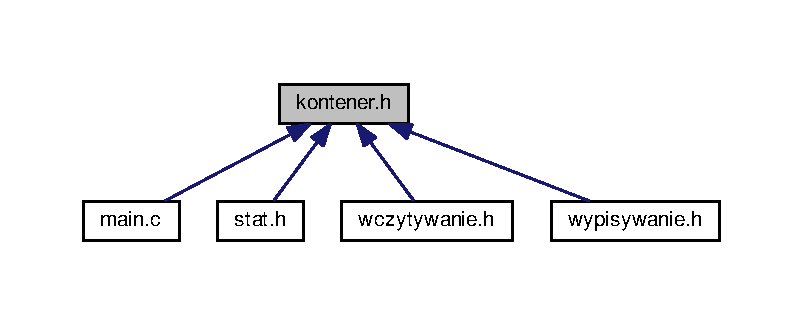
\includegraphics[width=350pt]{kontener_8h__dep__incl}
\end{center}
\end{figure}
\subsection*{Data Structures}
\begin{DoxyCompactItemize}
\item 
struct \hyperlink{structwej}{wej}
\item 
struct \hyperlink{structlokalizacja}{lokalizacja}
\item 
struct \hyperlink{structslowo}{slowo}
\item 
struct \hyperlink{structslownik}{slownik}
\end{DoxyCompactItemize}
\subsection*{Macros}
\begin{DoxyCompactItemize}
\item 
\#define \hyperlink{kontener_8h_a445e2870f22ce8f568d24b8d7212e76f}{S\+T\+A\+R\+T\+\_\+\+V\+E\+C}~2
\item 
\#define \hyperlink{kontener_8h_aaef6c04c23aa5ab59c7530d87e355c4e}{W\+R\+D\+\_\+\+M\+A\+X\+\_\+\+L\+E\+N\+G\+H\+T}~15
\item 
\#define \hyperlink{kontener_8h_a025aa7bcfdf6cb6964ab7e38fda249f5}{M\+A\+X\+\_\+\+F\+I\+L\+E\+\_\+\+D\+N}~100
\end{DoxyCompactItemize}
\subsection*{Typedefs}
\begin{DoxyCompactItemize}
\item 
typedef struct \hyperlink{structwej}{wej} \hyperlink{kontener_8h_a3810335f93d6bf3c564371621ce0ccb3}{wej\+\_\+t}
\item 
typedef struct \hyperlink{structlokalizacja}{lokalizacja} \hyperlink{kontener_8h_a973470f0d2bd5351f2f79b119fc095e8}{lok\+\_\+t}
\item 
typedef struct \hyperlink{structslowo}{slowo} \hyperlink{kontener_8h_aac4dfae9f3beb67b30cf6fd8ddb88731}{slowo\+\_\+t}
\item 
typedef struct \hyperlink{structslownik}{slownik} \hyperlink{kontener_8h_a9666b9a4046e295be733508d292247cc}{slownik\+\_\+t}
\end{DoxyCompactItemize}
\subsection*{Functions}
\begin{DoxyCompactItemize}
\item 
\hyperlink{kontener_8h_a3810335f93d6bf3c564371621ce0ccb3}{wej\+\_\+t} $\ast$ \hyperlink{kontener_8h_aa0d0bb7794d019bf8f8944253547cafe}{nowy\+\_\+wej} ()
\item 
\hyperlink{kontener_8h_a9666b9a4046e295be733508d292247cc}{slownik\+\_\+t} $\ast$ \hyperlink{kontener_8h_a7cfaed92dca5558f1ced9f66899e74dd}{pusty\+\_\+slownik} ()
\item 
int \hyperlink{kontener_8h_aa0d331daa9783130554097a06a21290f}{add\+\_\+slowo} (char $\ast$v)
\item 
\hyperlink{kontener_8h_a9666b9a4046e295be733508d292247cc}{slownik\+\_\+t} $\ast$ \hyperlink{kontener_8h_a91587cadf9ceb1dc80d35cee8b1f425e}{dodaj\+\_\+wystapienia} (\hyperlink{kontener_8h_a9666b9a4046e295be733508d292247cc}{slownik\+\_\+t} $\ast$\hyperlink{structslownik}{slownik}, char $\ast$$\ast$teksty)
\item 
\hyperlink{kontener_8h_a9666b9a4046e295be733508d292247cc}{slownik\+\_\+t} $\ast$ \hyperlink{kontener_8h_a913f9baec61bbbe5ec5257a0c5ca7aa8}{dodaj\+\_\+slowa} (\hyperlink{kontener_8h_a9666b9a4046e295be733508d292247cc}{slownik\+\_\+t} $\ast$\hyperlink{structslownik}{slownik}, char $\ast$$\ast$teksty, int ilosc\+\_\+tekstow)
\item 
\hyperlink{kontener_8h_a9666b9a4046e295be733508d292247cc}{slownik\+\_\+t} $\ast$ \hyperlink{kontener_8h_afa9c247f602e6c5684acb911f164d85c}{sortuj} (\hyperlink{kontener_8h_a9666b9a4046e295be733508d292247cc}{slownik\+\_\+t} $\ast$\hyperlink{structslownik}{slownik})
\item 
\hyperlink{kontener_8h_a9666b9a4046e295be733508d292247cc}{slownik\+\_\+t} $\ast$ \hyperlink{kontener_8h_a10f50b74340789cfce83113f4ee49c00}{polacz} (\hyperlink{kontener_8h_a9666b9a4046e295be733508d292247cc}{slownik\+\_\+t} $\ast$slownik\+\_\+z\+\_\+lok, \hyperlink{kontener_8h_a9666b9a4046e295be733508d292247cc}{slownik\+\_\+t} $\ast$slownik\+\_\+nowe\+\_\+slowa)
\item 
int \hyperlink{kontener_8h_ac345bd8eb624ab848da831c5b5059160}{add\+\_\+lok} (\hyperlink{kontener_8h_a9666b9a4046e295be733508d292247cc}{slownik\+\_\+t} $\ast$\hyperlink{structslownik}{slownik}, char $\ast$\hyperlink{structslowo}{slowo}, char $\ast$pref, char $\ast$suf)
\item 
int \hyperlink{kontener_8h_a9964976ca6ce4d2ebff3105e876ab97d}{daj\+\_\+indx} (\hyperlink{kontener_8h_a9666b9a4046e295be733508d292247cc}{slownik\+\_\+t} $\ast$\hyperlink{structslownik}{slownik}, char $\ast$\hyperlink{structslowo}{slowo})
\end{DoxyCompactItemize}


\subsection{Macro Definition Documentation}
\hypertarget{kontener_8h_a025aa7bcfdf6cb6964ab7e38fda249f5}{}\index{kontener.\+h@{kontener.\+h}!M\+A\+X\+\_\+\+F\+I\+L\+E\+\_\+\+D\+N@{M\+A\+X\+\_\+\+F\+I\+L\+E\+\_\+\+D\+N}}
\index{M\+A\+X\+\_\+\+F\+I\+L\+E\+\_\+\+D\+N@{M\+A\+X\+\_\+\+F\+I\+L\+E\+\_\+\+D\+N}!kontener.\+h@{kontener.\+h}}
\subsubsection[{M\+A\+X\+\_\+\+F\+I\+L\+E\+\_\+\+D\+N}]{\setlength{\rightskip}{0pt plus 5cm}\#define M\+A\+X\+\_\+\+F\+I\+L\+E\+\_\+\+D\+N~100}\label{kontener_8h_a025aa7bcfdf6cb6964ab7e38fda249f5}
Maksymalna długość nazwy i scierzki pliku \hypertarget{kontener_8h_a445e2870f22ce8f568d24b8d7212e76f}{}\index{kontener.\+h@{kontener.\+h}!S\+T\+A\+R\+T\+\_\+\+V\+E\+C@{S\+T\+A\+R\+T\+\_\+\+V\+E\+C}}
\index{S\+T\+A\+R\+T\+\_\+\+V\+E\+C@{S\+T\+A\+R\+T\+\_\+\+V\+E\+C}!kontener.\+h@{kontener.\+h}}
\subsubsection[{S\+T\+A\+R\+T\+\_\+\+V\+E\+C}]{\setlength{\rightskip}{0pt plus 5cm}\#define S\+T\+A\+R\+T\+\_\+\+V\+E\+C~2}\label{kontener_8h_a445e2870f22ce8f568d24b8d7212e76f}
początkowa ilość pól w wektorze \hypertarget{kontener_8h_aaef6c04c23aa5ab59c7530d87e355c4e}{}\index{kontener.\+h@{kontener.\+h}!W\+R\+D\+\_\+\+M\+A\+X\+\_\+\+L\+E\+N\+G\+H\+T@{W\+R\+D\+\_\+\+M\+A\+X\+\_\+\+L\+E\+N\+G\+H\+T}}
\index{W\+R\+D\+\_\+\+M\+A\+X\+\_\+\+L\+E\+N\+G\+H\+T@{W\+R\+D\+\_\+\+M\+A\+X\+\_\+\+L\+E\+N\+G\+H\+T}!kontener.\+h@{kontener.\+h}}
\subsubsection[{W\+R\+D\+\_\+\+M\+A\+X\+\_\+\+L\+E\+N\+G\+H\+T}]{\setlength{\rightskip}{0pt plus 5cm}\#define W\+R\+D\+\_\+\+M\+A\+X\+\_\+\+L\+E\+N\+G\+H\+T~15}\label{kontener_8h_aaef6c04c23aa5ab59c7530d87e355c4e}
maksymalna długość słowa 

\subsection{Typedef Documentation}
\hypertarget{kontener_8h_a973470f0d2bd5351f2f79b119fc095e8}{}\index{kontener.\+h@{kontener.\+h}!lok\+\_\+t@{lok\+\_\+t}}
\index{lok\+\_\+t@{lok\+\_\+t}!kontener.\+h@{kontener.\+h}}
\subsubsection[{lok\+\_\+t}]{\setlength{\rightskip}{0pt plus 5cm}typedef struct {\bf lokalizacja} {\bf lok\+\_\+t}}\label{kontener_8h_a973470f0d2bd5351f2f79b119fc095e8}
\hypertarget{kontener_8h_a9666b9a4046e295be733508d292247cc}{}\index{kontener.\+h@{kontener.\+h}!slownik\+\_\+t@{slownik\+\_\+t}}
\index{slownik\+\_\+t@{slownik\+\_\+t}!kontener.\+h@{kontener.\+h}}
\subsubsection[{slownik\+\_\+t}]{\setlength{\rightskip}{0pt plus 5cm}typedef struct {\bf slownik} {\bf slownik\+\_\+t}}\label{kontener_8h_a9666b9a4046e295be733508d292247cc}
\hypertarget{kontener_8h_aac4dfae9f3beb67b30cf6fd8ddb88731}{}\index{kontener.\+h@{kontener.\+h}!slowo\+\_\+t@{slowo\+\_\+t}}
\index{slowo\+\_\+t@{slowo\+\_\+t}!kontener.\+h@{kontener.\+h}}
\subsubsection[{slowo\+\_\+t}]{\setlength{\rightskip}{0pt plus 5cm}typedef struct {\bf slowo} {\bf slowo\+\_\+t}}\label{kontener_8h_aac4dfae9f3beb67b30cf6fd8ddb88731}
\hypertarget{kontener_8h_a3810335f93d6bf3c564371621ce0ccb3}{}\index{kontener.\+h@{kontener.\+h}!wej\+\_\+t@{wej\+\_\+t}}
\index{wej\+\_\+t@{wej\+\_\+t}!kontener.\+h@{kontener.\+h}}
\subsubsection[{wej\+\_\+t}]{\setlength{\rightskip}{0pt plus 5cm}typedef struct {\bf wej} {\bf wej\+\_\+t}}\label{kontener_8h_a3810335f93d6bf3c564371621ce0ccb3}


\subsection{Function Documentation}
\hypertarget{kontener_8h_ac345bd8eb624ab848da831c5b5059160}{}\index{kontener.\+h@{kontener.\+h}!add\+\_\+lok@{add\+\_\+lok}}
\index{add\+\_\+lok@{add\+\_\+lok}!kontener.\+h@{kontener.\+h}}
\subsubsection[{add\+\_\+lok}]{\setlength{\rightskip}{0pt plus 5cm}int add\+\_\+lok (
\begin{DoxyParamCaption}
\item[{{\bf slownik\+\_\+t} $\ast$}]{slownik, }
\item[{char $\ast$}]{slowo, }
\item[{char $\ast$}]{pref, }
\item[{char $\ast$}]{suf}
\end{DoxyParamCaption}
)}\label{kontener_8h_ac345bd8eb624ab848da831c5b5059160}
\hypertarget{kontener_8h_aa0d331daa9783130554097a06a21290f}{}\index{kontener.\+h@{kontener.\+h}!add\+\_\+slowo@{add\+\_\+slowo}}
\index{add\+\_\+slowo@{add\+\_\+slowo}!kontener.\+h@{kontener.\+h}}
\subsubsection[{add\+\_\+slowo}]{\setlength{\rightskip}{0pt plus 5cm}int add\+\_\+slowo (
\begin{DoxyParamCaption}
\item[{char $\ast$}]{v}
\end{DoxyParamCaption}
)}\label{kontener_8h_aa0d331daa9783130554097a06a21290f}
\hypertarget{kontener_8h_a9964976ca6ce4d2ebff3105e876ab97d}{}\index{kontener.\+h@{kontener.\+h}!daj\+\_\+indx@{daj\+\_\+indx}}
\index{daj\+\_\+indx@{daj\+\_\+indx}!kontener.\+h@{kontener.\+h}}
\subsubsection[{daj\+\_\+indx}]{\setlength{\rightskip}{0pt plus 5cm}int daj\+\_\+indx (
\begin{DoxyParamCaption}
\item[{{\bf slownik\+\_\+t} $\ast$}]{slownik, }
\item[{char $\ast$}]{slowo}
\end{DoxyParamCaption}
)}\label{kontener_8h_a9964976ca6ce4d2ebff3105e876ab97d}
\hypertarget{kontener_8h_a913f9baec61bbbe5ec5257a0c5ca7aa8}{}\index{kontener.\+h@{kontener.\+h}!dodaj\+\_\+slowa@{dodaj\+\_\+slowa}}
\index{dodaj\+\_\+slowa@{dodaj\+\_\+slowa}!kontener.\+h@{kontener.\+h}}
\subsubsection[{dodaj\+\_\+slowa}]{\setlength{\rightskip}{0pt plus 5cm}{\bf slownik\+\_\+t}$\ast$ dodaj\+\_\+slowa (
\begin{DoxyParamCaption}
\item[{{\bf slownik\+\_\+t} $\ast$}]{slownik, }
\item[{char $\ast$$\ast$}]{teksty, }
\item[{int}]{ilosc\+\_\+tekstow}
\end{DoxyParamCaption}
)}\label{kontener_8h_a913f9baec61bbbe5ec5257a0c5ca7aa8}
\hypertarget{kontener_8h_a91587cadf9ceb1dc80d35cee8b1f425e}{}\index{kontener.\+h@{kontener.\+h}!dodaj\+\_\+wystapienia@{dodaj\+\_\+wystapienia}}
\index{dodaj\+\_\+wystapienia@{dodaj\+\_\+wystapienia}!kontener.\+h@{kontener.\+h}}
\subsubsection[{dodaj\+\_\+wystapienia}]{\setlength{\rightskip}{0pt plus 5cm}{\bf slownik\+\_\+t}$\ast$ dodaj\+\_\+wystapienia (
\begin{DoxyParamCaption}
\item[{{\bf slownik\+\_\+t} $\ast$}]{slownik, }
\item[{char $\ast$$\ast$}]{teksty}
\end{DoxyParamCaption}
)}\label{kontener_8h_a91587cadf9ceb1dc80d35cee8b1f425e}
\hypertarget{kontener_8h_aa0d0bb7794d019bf8f8944253547cafe}{}\index{kontener.\+h@{kontener.\+h}!nowy\+\_\+wej@{nowy\+\_\+wej}}
\index{nowy\+\_\+wej@{nowy\+\_\+wej}!kontener.\+h@{kontener.\+h}}
\subsubsection[{nowy\+\_\+wej}]{\setlength{\rightskip}{0pt plus 5cm}{\bf wej\+\_\+t}$\ast$ nowy\+\_\+wej (
\begin{DoxyParamCaption}
{}
\end{DoxyParamCaption}
)}\label{kontener_8h_aa0d0bb7794d019bf8f8944253547cafe}
\hypertarget{kontener_8h_a10f50b74340789cfce83113f4ee49c00}{}\index{kontener.\+h@{kontener.\+h}!polacz@{polacz}}
\index{polacz@{polacz}!kontener.\+h@{kontener.\+h}}
\subsubsection[{polacz}]{\setlength{\rightskip}{0pt plus 5cm}{\bf slownik\+\_\+t}$\ast$ polacz (
\begin{DoxyParamCaption}
\item[{{\bf slownik\+\_\+t} $\ast$}]{slownik\+\_\+z\+\_\+lok, }
\item[{{\bf slownik\+\_\+t} $\ast$}]{slownik\+\_\+nowe\+\_\+slowa}
\end{DoxyParamCaption}
)}\label{kontener_8h_a10f50b74340789cfce83113f4ee49c00}
\hypertarget{kontener_8h_a7cfaed92dca5558f1ced9f66899e74dd}{}\index{kontener.\+h@{kontener.\+h}!pusty\+\_\+slownik@{pusty\+\_\+slownik}}
\index{pusty\+\_\+slownik@{pusty\+\_\+slownik}!kontener.\+h@{kontener.\+h}}
\subsubsection[{pusty\+\_\+slownik}]{\setlength{\rightskip}{0pt plus 5cm}{\bf slownik\+\_\+t}$\ast$ pusty\+\_\+slownik (
\begin{DoxyParamCaption}
{}
\end{DoxyParamCaption}
)}\label{kontener_8h_a7cfaed92dca5558f1ced9f66899e74dd}
\hypertarget{kontener_8h_afa9c247f602e6c5684acb911f164d85c}{}\index{kontener.\+h@{kontener.\+h}!sortuj@{sortuj}}
\index{sortuj@{sortuj}!kontener.\+h@{kontener.\+h}}
\subsubsection[{sortuj}]{\setlength{\rightskip}{0pt plus 5cm}{\bf slownik\+\_\+t}$\ast$ sortuj (
\begin{DoxyParamCaption}
\item[{{\bf slownik\+\_\+t} $\ast$}]{slownik}
\end{DoxyParamCaption}
)}\label{kontener_8h_afa9c247f602e6c5684acb911f164d85c}

\hypertarget{main_8c}{}\section{main.\+c File Reference}
\label{main_8c}\index{main.\+c@{main.\+c}}
{\ttfamily \#include $<$stdio.\+h$>$}\\*
{\ttfamily \#include $<$string.\+h$>$}\\*
{\ttfamily \#include \char`\"{}kontener.\+h\char`\"{}}\\*
Include dependency graph for main.\+c\+:\nopagebreak
\begin{figure}[H]
\begin{center}
\leavevmode
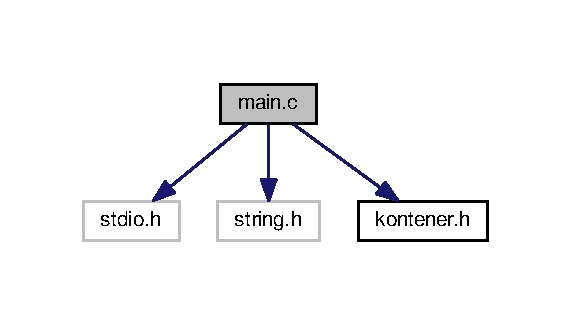
\includegraphics[width=274pt]{main_8c__incl}
\end{center}
\end{figure}
\subsection*{Functions}
\begin{DoxyCompactItemize}
\item 
int \hyperlink{main_8c_a3c04138a5bfe5d72780bb7e82a18e627}{main} (int argc, char $\ast$$\ast$argv)
\end{DoxyCompactItemize}


\subsection{Function Documentation}
\hypertarget{main_8c_a3c04138a5bfe5d72780bb7e82a18e627}{}\index{main.\+c@{main.\+c}!main@{main}}
\index{main@{main}!main.\+c@{main.\+c}}
\subsubsection[{main}]{\setlength{\rightskip}{0pt plus 5cm}int main (
\begin{DoxyParamCaption}
\item[{int}]{argc, }
\item[{char $\ast$$\ast$}]{argv}
\end{DoxyParamCaption}
)}\label{main_8c_a3c04138a5bfe5d72780bb7e82a18e627}
Funkcja sterująca programem 
\begin{DoxyParams}{Parameters}
{\em argc} & -\/ile jest parametrów uruchomienia \\
\hline
{\em argv} & -\/parametry uruchomienia \\
\hline
\end{DoxyParams}
\begin{DoxyReturn}{Returns}
0 
\end{DoxyReturn}

\hypertarget{stat_8h}{}\section{stat.\+h File Reference}
\label{stat_8h}\index{stat.\+h@{stat.\+h}}
{\ttfamily \#include \char`\"{}kontener.\+h\char`\"{}}\\*
Include dependency graph for stat.\+h\+:\nopagebreak
\begin{figure}[H]
\begin{center}
\leavevmode
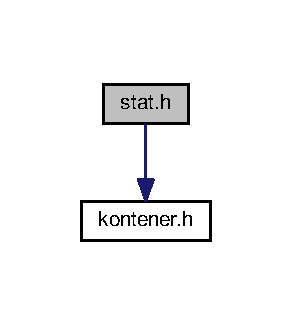
\includegraphics[width=140pt]{stat_8h__incl}
\end{center}
\end{figure}
\subsection*{Functions}
\begin{DoxyCompactItemize}
\item 
char $\ast$$\ast$ \hyperlink{stat_8h_af039248e0f998eb2e758f3b5d1a48ac5}{max\+\_\+slowo} (\hyperlink{kontener_8h_a9666b9a4046e295be733508d292247cc}{slownik\+\_\+t} $\ast$\hyperlink{structslownik}{slownik})
\item 
char $\ast$$\ast$ \hyperlink{stat_8h_ac8c3cb028bb0b4c604c6514992606c73}{max\+\_\+gram} (\hyperlink{kontener_8h_a9666b9a4046e295be733508d292247cc}{slownik\+\_\+t} $\ast$\hyperlink{structslownik}{slownik}, int n)
\end{DoxyCompactItemize}


\subsection{Function Documentation}
\hypertarget{stat_8h_ac8c3cb028bb0b4c604c6514992606c73}{}\index{stat.\+h@{stat.\+h}!max\+\_\+gram@{max\+\_\+gram}}
\index{max\+\_\+gram@{max\+\_\+gram}!stat.\+h@{stat.\+h}}
\subsubsection[{max\+\_\+gram}]{\setlength{\rightskip}{0pt plus 5cm}char$\ast$$\ast$ max\+\_\+gram (
\begin{DoxyParamCaption}
\item[{{\bf slownik\+\_\+t} $\ast$}]{slownik, }
\item[{int}]{n}
\end{DoxyParamCaption}
)}\label{stat_8h_ac8c3cb028bb0b4c604c6514992606c73}
\hypertarget{stat_8h_af039248e0f998eb2e758f3b5d1a48ac5}{}\index{stat.\+h@{stat.\+h}!max\+\_\+slowo@{max\+\_\+slowo}}
\index{max\+\_\+slowo@{max\+\_\+slowo}!stat.\+h@{stat.\+h}}
\subsubsection[{max\+\_\+slowo}]{\setlength{\rightskip}{0pt plus 5cm}char$\ast$$\ast$ max\+\_\+slowo (
\begin{DoxyParamCaption}
\item[{{\bf slownik\+\_\+t} $\ast$}]{slownik}
\end{DoxyParamCaption}
)}\label{stat_8h_af039248e0f998eb2e758f3b5d1a48ac5}

\hypertarget{wczytywanie_8h}{}\section{wczytywanie.\+h File Reference}
\label{wczytywanie_8h}\index{wczytywanie.\+h@{wczytywanie.\+h}}
{\ttfamily \#include \char`\"{}kontener.\+h\char`\"{}}\\*
Include dependency graph for wczytywanie.\+h\+:\nopagebreak
\begin{figure}[H]
\begin{center}
\leavevmode
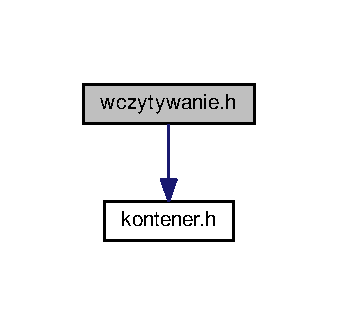
\includegraphics[width=162pt]{wczytywanie_8h__incl}
\end{center}
\end{figure}
\subsection*{Functions}
\begin{DoxyCompactItemize}
\item 
\hyperlink{kontener_8h_a9666b9a4046e295be733508d292247cc}{slownik\+\_\+t} $\ast$ \hyperlink{wczytywanie_8h_a3c899387445428d62ba9d72bca8f381f}{wczytaj\+\_\+slownik} (char $\ast$baza)
\item 
\hyperlink{kontener_8h_a9666b9a4046e295be733508d292247cc}{slownik\+\_\+t} $\ast$ \hyperlink{wczytywanie_8h_a1fb1da2cf18edd38dac3be29deeaf741}{powieksz\+\_\+slownik} (char $\ast$baza, char $\ast$$\ast$teksty)
\end{DoxyCompactItemize}


\subsection{Function Documentation}
\hypertarget{wczytywanie_8h_a1fb1da2cf18edd38dac3be29deeaf741}{}\index{wczytywanie.\+h@{wczytywanie.\+h}!powieksz\+\_\+slownik@{powieksz\+\_\+slownik}}
\index{powieksz\+\_\+slownik@{powieksz\+\_\+slownik}!wczytywanie.\+h@{wczytywanie.\+h}}
\subsubsection[{powieksz\+\_\+slownik}]{\setlength{\rightskip}{0pt plus 5cm}{\bf slownik\+\_\+t}$\ast$ powieksz\+\_\+slownik (
\begin{DoxyParamCaption}
\item[{char $\ast$}]{baza, }
\item[{char $\ast$$\ast$}]{teksty}
\end{DoxyParamCaption}
)}\label{wczytywanie_8h_a1fb1da2cf18edd38dac3be29deeaf741}
\hypertarget{wczytywanie_8h_a3c899387445428d62ba9d72bca8f381f}{}\index{wczytywanie.\+h@{wczytywanie.\+h}!wczytaj\+\_\+slownik@{wczytaj\+\_\+slownik}}
\index{wczytaj\+\_\+slownik@{wczytaj\+\_\+slownik}!wczytywanie.\+h@{wczytywanie.\+h}}
\subsubsection[{wczytaj\+\_\+slownik}]{\setlength{\rightskip}{0pt plus 5cm}{\bf slownik\+\_\+t}$\ast$ wczytaj\+\_\+slownik (
\begin{DoxyParamCaption}
\item[{char $\ast$}]{baza}
\end{DoxyParamCaption}
)}\label{wczytywanie_8h_a3c899387445428d62ba9d72bca8f381f}

\hypertarget{wypisywanie_8h}{}\section{wypisywanie.\+h File Reference}
\label{wypisywanie_8h}\index{wypisywanie.\+h@{wypisywanie.\+h}}
{\ttfamily \#include \char`\"{}kontener.\+h\char`\"{}}\\*
Include dependency graph for wypisywanie.\+h\+:\nopagebreak
\begin{figure}[H]
\begin{center}
\leavevmode
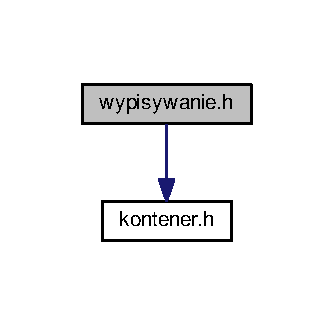
\includegraphics[width=160pt]{wypisywanie_8h__incl}
\end{center}
\end{figure}
\subsection*{Functions}
\begin{DoxyCompactItemize}
\item 
int \hyperlink{wypisywanie_8h_a4145a0c06b371fd1553f39ea507ae5f5}{wyp\+\_\+sl} (\hyperlink{kontener_8h_a9666b9a4046e295be733508d292247cc}{slownik\+\_\+t} $\ast$\hyperlink{structslownik}{slownik}, char $\ast$scierzka)
\item 
int \hyperlink{wypisywanie_8h_a5dadb04155d3d69c56eb757d39ee500b}{gen\+\_\+t} (int slowa, int akapity, char $\ast$plik, \hyperlink{kontener_8h_a9666b9a4046e295be733508d292247cc}{slownik\+\_\+t} $\ast$\hyperlink{structslownik}{slownik})
\item 
int \hyperlink{wypisywanie_8h_ab3f6393f95a5dbfb039c9a23c54ba497}{gen\+\_\+stat} (\hyperlink{kontener_8h_a9666b9a4046e295be733508d292247cc}{slownik\+\_\+t} $\ast$\hyperlink{structslownik}{slownik})
\end{DoxyCompactItemize}


\subsection{Function Documentation}
\hypertarget{wypisywanie_8h_ab3f6393f95a5dbfb039c9a23c54ba497}{}\index{wypisywanie.\+h@{wypisywanie.\+h}!gen\+\_\+stat@{gen\+\_\+stat}}
\index{gen\+\_\+stat@{gen\+\_\+stat}!wypisywanie.\+h@{wypisywanie.\+h}}
\subsubsection[{gen\+\_\+stat}]{\setlength{\rightskip}{0pt plus 5cm}int gen\+\_\+stat (
\begin{DoxyParamCaption}
\item[{{\bf slownik\+\_\+t} $\ast$}]{slownik}
\end{DoxyParamCaption}
)}\label{wypisywanie_8h_ab3f6393f95a5dbfb039c9a23c54ba497}
\hypertarget{wypisywanie_8h_a5dadb04155d3d69c56eb757d39ee500b}{}\index{wypisywanie.\+h@{wypisywanie.\+h}!gen\+\_\+t@{gen\+\_\+t}}
\index{gen\+\_\+t@{gen\+\_\+t}!wypisywanie.\+h@{wypisywanie.\+h}}
\subsubsection[{gen\+\_\+t}]{\setlength{\rightskip}{0pt plus 5cm}int gen\+\_\+t (
\begin{DoxyParamCaption}
\item[{int}]{slowa, }
\item[{int}]{akapity, }
\item[{char $\ast$}]{plik, }
\item[{{\bf slownik\+\_\+t} $\ast$}]{slownik}
\end{DoxyParamCaption}
)}\label{wypisywanie_8h_a5dadb04155d3d69c56eb757d39ee500b}
\hypertarget{wypisywanie_8h_a4145a0c06b371fd1553f39ea507ae5f5}{}\index{wypisywanie.\+h@{wypisywanie.\+h}!wyp\+\_\+sl@{wyp\+\_\+sl}}
\index{wyp\+\_\+sl@{wyp\+\_\+sl}!wypisywanie.\+h@{wypisywanie.\+h}}
\subsubsection[{wyp\+\_\+sl}]{\setlength{\rightskip}{0pt plus 5cm}int wyp\+\_\+sl (
\begin{DoxyParamCaption}
\item[{{\bf slownik\+\_\+t} $\ast$}]{slownik, }
\item[{char $\ast$}]{scierzka}
\end{DoxyParamCaption}
)}\label{wypisywanie_8h_a4145a0c06b371fd1553f39ea507ae5f5}
zapisuje słownik do pliku 
%--- End generated contents ---

% Index
\backmatter
\newpage
\phantomsection
\clearemptydoublepage
\addcontentsline{toc}{chapter}{Index}
\printindex

\end{document}
